%%%%%%%%%%%%%%%%%%%%%%%%%%%%%%%%%%%%%%%%%%%%%%%%%
%%%%%%%%%%%% chap: architecture %%%%%%%%%%%%%%%%%
%%%%%%%%%%%%%%%%%%%%%%%%%%%%%%%%%%%%%%%%%%%%%%%%%

\chapter{Architecture}\label{chapter:Architecture}

%%%%%%%%%%%% Section: Use Case %%%%%%%%%%%%
\section{Use Cases}\label{sect:use cases}
\vspace{20pt}
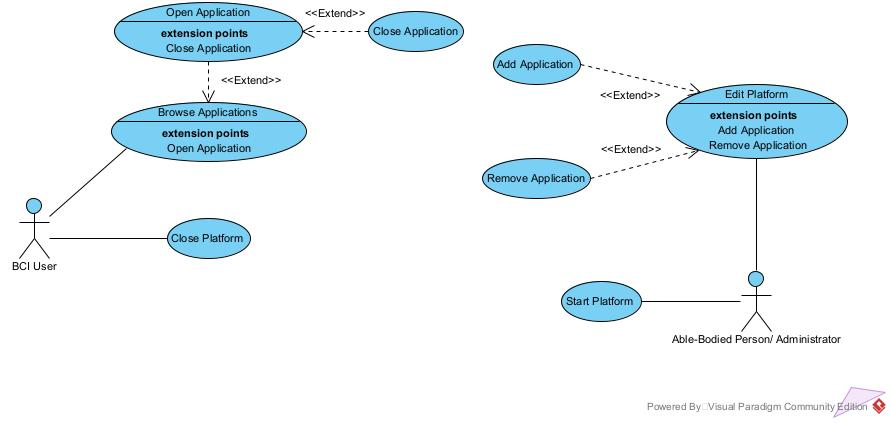
\includegraphics[width = 420pt]{Diagrams/Use Case.jpg}

\hspace{\parindent} The app will primarily be used by 2 categories of users: BCI users and able-bodied users/app administrators. BCI users will be the actual users of the app while the administrators' role will be maintenance or starting the application. 

\hspace{\parindent} The BCI users can use the platform through the brain computer interface. They can choose from a selection of different applications using a intuitive graphical user interface provided by the platform. Once selected, the application may be used indefinitely or until the user decides he/she is done with it, at which point the app may be closed by the users, bringing them back to the main page of the platform. Alongside using the applications, the user may also close the platform altogether. In the case of patients that cannot talk, this can be useful to signal a caretaker that they are done for the day.

\hspace{\parindent} The app administrator or generally any able-bodied person with knowledge of the platform can edit the apps housed by said platform at any time, adding or removing applications accordingly. They may also start the platform, since a BCI user without motor skills cannot do this by their own volition.


%%%%%%%%%%%% Section: Architectural Schematic %%%%%%%%%%%%
\section{Architectural Schematic}\label{sect:architectural schematic}
\vspace{20pt}
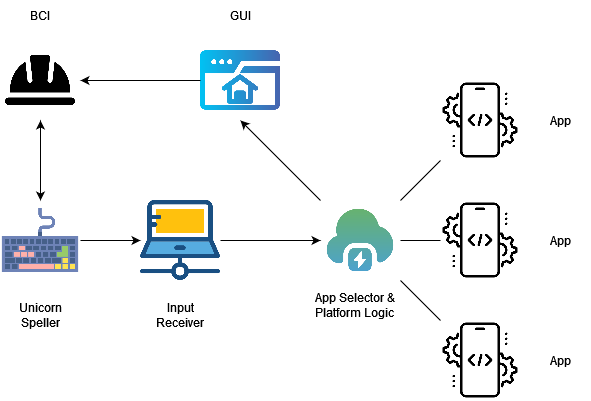
\includegraphics[width = 420pt]{Diagrams/Architectural.png}

\hspace{\parindent} The main point of the app architecture is the Brain Computer interface itself. Through it the user can communicate with the Unicorn Speller, the proprietary software created by Unicorn to allow disabled people to communicate. Using the same software and a receiver we can take signals from the users and process them as actions inside the platform. At which point the platform makes the necessary changes to the GUI that the user sees and communicates accordingly with one of the applications housed in the platform, if the user selected one.